\documentclass[12pt]{article}
\usepackage{amsmath}
\usepackage{amssymb}
\usepackage{graphicx}
\usepackage{tabulary}
\usepackage{float}
\usepackage{hyperref}

\begin{document}

\title{Homework 1 for Einstein group}%replace X with the appropriate number
\author{William Harrington, David Hernandez, Waleed Alhaddad\\ %replace with your name
ECE478} %if necessary, replace with your course title
\date{}
 
\maketitle
\small
\begin{description}
	\item[Introduction] \hfill \\ \\
		This report contains a detailed explanation of the homework 1 assignment for the Einstein group. \\ \\
		\textbf{Learning Outcomes} \\
		The purpose of this homework was to fulfill the following learning outcomes.
		\begin{enumerate}
			\item Use of Kinect to control a robot, to create commands and data for a robot.
			\item The concept of state machine in robotics
			\item The concept and use of fuzzy logic in robotics
			\item Using Powerpoint for scenario prototyping
			\item Dialogs with robots
		\end{enumerate}
		\newpage
		\textbf{First phase explanation}
		\begin{figure}[H]
			\centering
			\caption{A high level diagram of the first phase objectives}
			\fbox{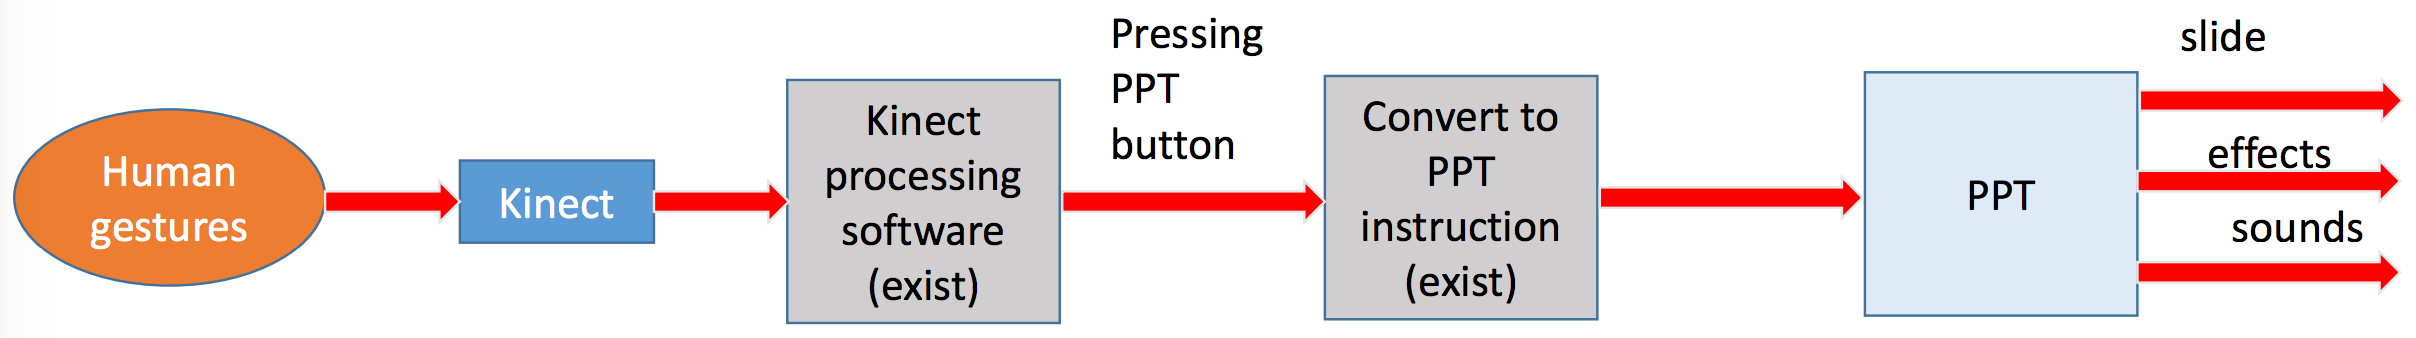
\includegraphics[scale=.3]{hw1_phase1_diagram.png}}
		\end{figure}
		\textbf{The objective for the first phase of this homework was to:}
		\begin{enumerate}
			\item Figure out how to use a Kinect to control the mouse on a computer 
			\item Figure out how to use Kinect to control a powerpoint presentation
			\item Create a powerpoint presentation with info, effects, figures, pictures, and videos about Einstein and the "Quantum Debate" play
			\item Record voice with German accent that is suppose to be Einstein for the powerpoint presentation
		\end{enumerate}
		In order to meet these objectives, our group did the following:
		\begin{itemize}
			\item We created a powerpoint presentation using Microsoft Powerpoint.
				\begin{itemize}
					\item The powerpoint presentation contains
						\begin{itemize}
							\item Famous quotes from Einstein
							\item History about Einstein's life, achievements, and hobbies
							\item Einstein's parts in the "Great Quantum Debate", Acts I and II
							\item Lots of pictures of Einstein himself and things related to him
							\item A voice with a german accent that reads what is on the slide
						\end{itemize}
					\item Within the powerpoint presentation, several macros were created using Microsoft Visual Basic for Applications.
						\begin{itemize}
							\item Macros were used to make buttons that could be clicked on with the mouse to transition to another slide
						\end{itemize}
				\end{itemize}
			\newpage
			\item We found software called KinectMouse for controlling a PC mouse and powerpoint presentation with Kinect
				\begin{itemize}
					\item The software can be located \href{https://kinectmouse.codeplex.com/}{here} \footnote{https://kinectmouse.codeplex.com/}
					\item There are detailed instructions on how to use this software \href{http://futuretechblog.com/?p=26}{here} \footnote{http://futuretechblog.com/?p=26}
					\item We also found a tutorial on how to use a face to control the mouse with this software \href{http://futuretechblog.com/?p=71}{here} \footnote{http://futuretechblog.com/?p=71} but never had time to implement it
				\end{itemize}
			\item We found a website that does text to sound in many different accents performed by either a male or a female voice called \textbf{IVONA}\footnote{https://www.ivona.com/}
				\begin{itemize}
					\item We used the male German accent to suit our robot Einstein
					\item We needed to record the sound internally to have a better quality sound, so we used a program called \textbf{Audacity}\footnote{http://www.audacityteam.org/}
					\item We edited the recorded scripts by using a program called \textbf{Mixxx}\footnote{http://mixxx.org/}
					\item All the programs the we used for the sound are available free online
				\end{itemize}
		\end{itemize}
		\textbf{Group roles for first phase}
		\begin{itemize}
			\item Powerpoint: Will, David, Waleed
			\item KinectMouse: David
			\item Voice effects: Waleed
			\item Documentation: Will
		\end{itemize} \hfill \\
		\newpage
		\textbf{Second phase explanation}
		\begin{figure}[H]
			\centering
			\caption{A high level diagram of the second phase objectives}
			\fbox{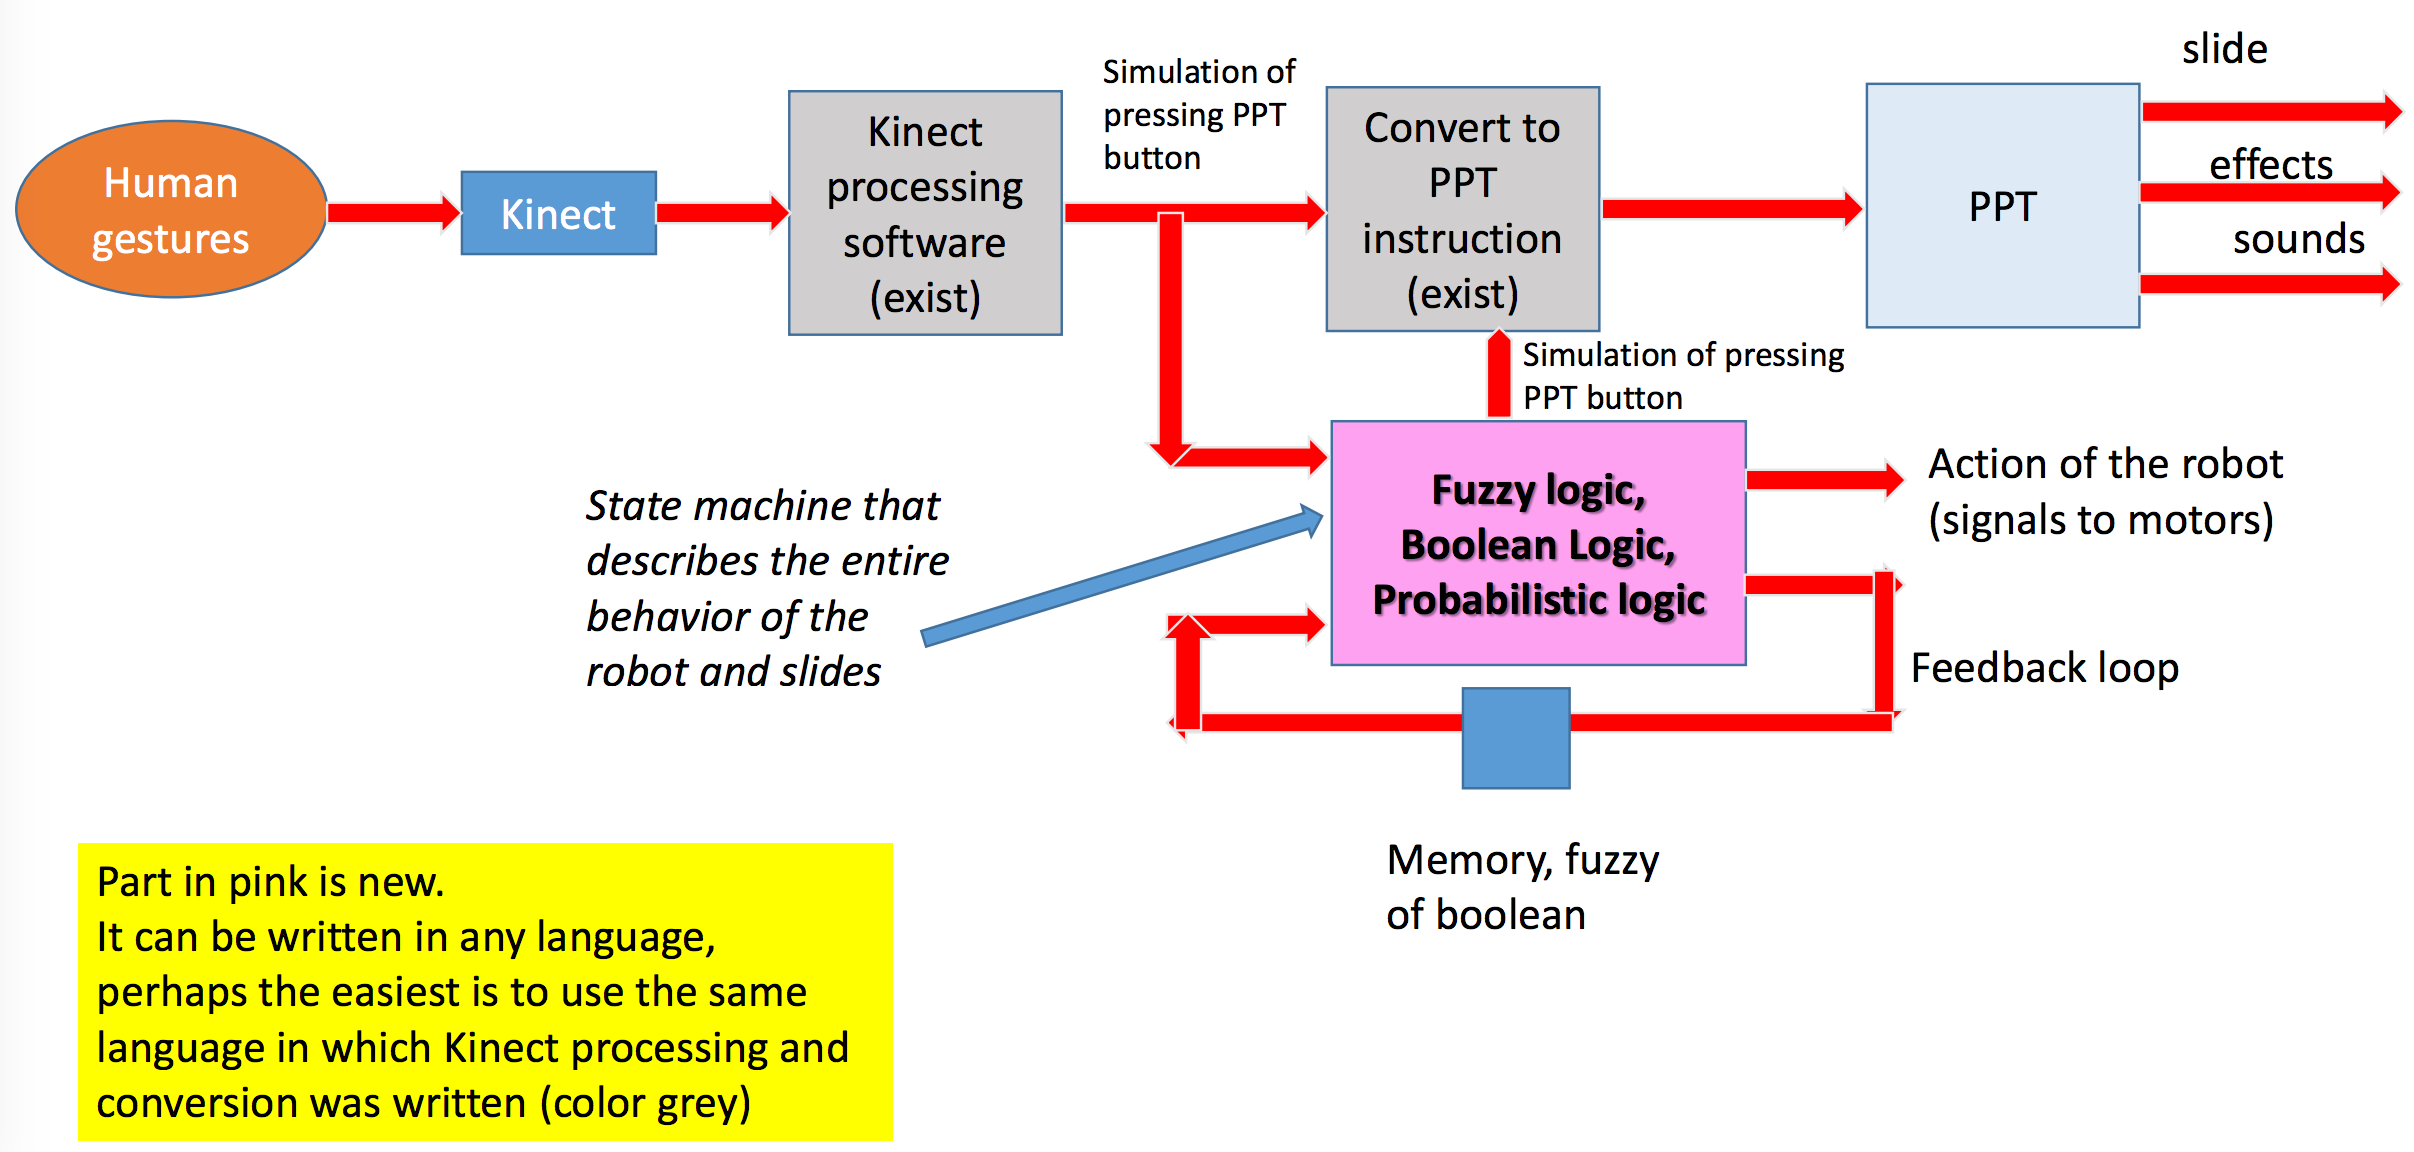
\includegraphics[scale=.25]{hw1_phase2_diagram.png}}
		\end{figure}
		\textbf{The objective for the second phase of this homework was to:}
		\begin{enumerate}
			\item Create a state machine in software that describes the behavior of the robot, robots, and/or the entire theatre presentation
				\begin{itemize}
					\item Could be deterministic, probabilistic, or fuzzy, or a mix of these.
					\item Can have several machines communicating with one another.
					\item Can be programmed in any language.
					\item Should use Microsoft Powerpoint and Kinect software
				\end{itemize} 
			\item Record a video demonstration
		\end{enumerate}
		In order to meet these objectives, our group did the following:
		\begin{itemize}
			\item We chose to use python for programming the state machine
			%\newpage
			\item A python class object was created to describe the behavior of the Einstein robot
				\begin{itemize}
					\item It is appropriately titled "Einstein"
					\item It can be found \href{https://github.com/wrh2/ECE478/blob/master/Einstein/Einstein.py}{here} \footnote{https://github.com/wrh2/ECE478/blob/master/Einstein/Einstein.py}
					\item It contains multiple ways to potentially control the behavior of the robot
					\item The behavior of the robot is determined by probabilistic logic using random number generators
				\end{itemize}
			\newpage
			\item A python program was made to demonstrate the python class object
				\begin{itemize}
					\item It is called "main"
					\item It can be found \href{https://github.com/wrh2/ECE478/blob/master/Einstein/main.py}{here} \footnote{https://github.com/wrh2/ECE478/blob/master/Einstein/main.py}
					\item It takes arguments from the command line, parses them and then calls the appropriate method in the Einstein python class object
						\begin{itemize}
							\item Code requires the following python libraries to run: argparse, random, Einstein.py (see footnotes on page 4)
							\item There is also a README located \href{https://github.com/wrh2/ECE478/blob/master/Einstein/README.md}{here} \footnote{https://github.com/wrh2/ECE478/blob/master/Einstein/README.md}
						\end{itemize}
				\end{itemize}
			\item We introduced more macros within the powerpoint presentation 
				\begin{itemize}
					\item Some of them exhibit probabilistic logic (i.e. randomly choosing slides)
					\item Some of them interface with the Python code
					\item All buttons that are connected to macros were labelled accordingly
				\end{itemize}
			\item We recorded a video demonstration of our project
				\begin{itemize}
					\item Shows the use of the Kinect software to control the mouse and powerpoint
					\item Shows effects and voices in powerpoint presentation
					\item Shows the interaction between the powerpoint and python software
				\end{itemize}
		\end{itemize}
		\textbf{Group roles for second phase}
		\begin{itemize}
			\item Powerpoint: Will, David, Waleed
			\item Powerpoint macros: David
			\item Python programming: Will
			\item Video recording/editing: David, Will
			\item Documentation: Will
		\end{itemize} \hfill \\
		\newpage
		\textbf{Results}
		\begin{itemize}
			\item Successfully used Kinect to control mouse and powerpoint presentation
			\item Successfully demonstrated interaction between powerpoint presentation and python code
			\item Showcased fun and interesting information about Einstein using voice effects, images, and sounds in powerpoint
			\item All materials (presentation, video, report, code) can be found \href{https://github.com/wrh2/ECE478/tree/master/Einstein}{here} \footnote{https://github.com/wrh2/ECE478/tree/master/Einstein}
		\end{itemize}
		
\end{description}

\end{document}